\documentclass{report}
% \documentclass{article}
\usepackage{graphicx} % Required for inserting images
\usepackage{hyperref} % Required for links

\graphicspath{ {./images/} }

\title{Report about AdamW and Muon optimizers comparison}
\author{Kabanov D.S.}
\date{March 2026}

\begin{document}

\maketitle % Generates the title page

\tableofcontents % Generates the Table of Contents (compile twice to update)

\chapter{Task definition}
Recently, the \href{https://github.com/MoonshotAI/Moonlight}{Muon optimizer}, based on matrix orthogonalization, has demonstrated strong results in scaling the training process from small language models to larger models and achieving 2× computational efficiency compared to AdamW. 
The task is to perform a comparison of recent optimization strategies (\href{https://docs.pytorch.org/docs/stable/generated/torch.optim.AdamW.html}{AdamW}, \href{https://docs.pytorch.org/docs/stable/generated/torch.optim.Muon.html}{Muon}) by \textbf{training time}, \textbf{maximum memory usage}, \textbf{final model quality}, and \textbf{training convergence}:
\begin{enumerate}
    \item Download:
        \begin{itemize}
        \item From Hugging Face: \href{https://huggingface.co/Qwen/Qwen2.5-0.5B}{Qwen2.5-0.5B} model, training dataset \href{https://huggingface.co/datasets/Elriggs/openwebtext-100k}{openwebtext-100k};
        \item From GitHub: evaluation \href{https://github.com/EleutherAI/lm-evaluation-harness}{benchmarks} (piqa, arc\_easy, arc\_challenge, winogrande, hellaswag) and \href{https://github.com/princeton-nlp/MeZO}{MeZO} optimizer if you want a challenge.
        \end{itemize}
    \item Perform \textbf{full fine-tuning} of the model with the following optimizers (using at least 1% of training dataset):
        \begin{itemize}
        \item \href{https://docs.pytorch.org/docs/stable/generated/torch.optim.AdamW.html}{AdamW};
        \item \href{https://docs.pytorch.org/docs/stable/generated/torch.optim.Muon.html}{Muon};
        \item Improve  Muon  quality  with  a  combination  of  Muon  and  AdamW.  Model parameters are split into 2 groups. The first part of the model is trained with Muon, and the second part is trained with AdamW;
        \item \textit{\textbf{[Challenge]}} \href{https://github.com/princeton-nlp/MeZO}{MeZO}.
        \end{itemize}
    \item Compare  \textbf{training speed},  \textbf{GPU memory usage}, \textbf{quality} of finetuned models and \textbf{training convergence}.
    \item Present a report in LaTeX format.
\end{enumerate}

\textit{Publish the solution as a public repository on GitHub. The report should be presented as a LaTeX document. Instructions should be presented in README.md.}


\chapter{Algorithms description}
\section{AdamW}
\textbf{Adam} optimizer (Adaptive Moment Estimation) — an algorithm for optimizing the weights of neural networks based on the backpropagation of error (gradient) and combining ideas from Nesterov Accelerated Gradient (\textit{\textbf{Momentum}}) and RMSProp (\textit{\textbf{individual step for each parameter}}). \textit{The algorithm stores in memory two moments (matrices) \textbf{for each trainable parameter} of the model}:

1. The first moment (aka the moving average of the gradient, $m_t$) is an analogue of Momentum, which helps not to get stuck in local minima.

2. The second moment (aka the moving average of the square of the gradient, $v_t$) is an analogue of adaptive velocity, it helps to reduce the step where the gradients are very sharp and increase where they are flat.

Their combination allows the optimizer to take larger steps on flat terrain and smaller, careful steps on steep or "noisy" terrain.
\\\\
\textit{\textbf{Adam algorithm}} consists of the following steps (at each iteration $t$, the following calculations are performed for each parameter $\theta$):

0) Initially, at $t=0$, moments $m_t$ (or $m_0$) and $v_t$ (or $v_0$) for the weight matrices are zero.

1) The gradient $g_t$ (the derivative of the loss function with respect to the current weight $\theta$) is calculated using the formula:
    $$g_t = \nabla_{\theta}L(\theta_t)$$

        \textbf{If L2-regularization is applied} ($\lambda$ is the regularization coefficient, weight decay), then the gradient of $g_t$ is considered as:
    $$g_t = \nabla_{\theta}L(\theta_t) + \lambda \cdot \theta_{t}$$
    
2) The moments are updated (using exponential attenuation $\sim$ so that the "old" gradients are forgotten and the "new" ones have more weight):
    $$m_t = \beta_1 \cdot m_{t-1} + (1 - \beta_1) \cdot g_t$$
    $$v_t = \beta_2 \cdot v_{t-1} + (1 - \beta_2) \cdot g_t^2$$

    $\beta_1$ (usually 0.9) determines how much we trust past experience. $\beta_2$ (usually 0.999) is responsible for the "memory" of gradient volatility.
    
3) Bias Correction. Due to the fact that at the very beginning of training $m_t$ and $v_t$ are equal to 0, they "accelerate" for a long time and tend to zero. To fix this, they are scaled (due to which, for small $t>0$, their values are several times larger than they should be, but as $t$ increases, $\beta^t$ decreases, and therefore the scaling factor tends to 1):
    $$\hat{m}_t = \frac{m_t}{1-\beta_1^t}$$
    $$\hat{v}_t = \frac{v_t}{1-\beta_2^t}$$
    
4) After scaling, the model weights are updated ($\eta$ — learning rate, $\epsilon$ — minimum addition so that there is no zero in the denominator):
    $$\theta_{t+1} = \theta_t - \eta \cdot \frac{\hat{m}_t}{\sqrt{\hat{v}_t} + \epsilon}$$
\begin{figure}[h]
\centering
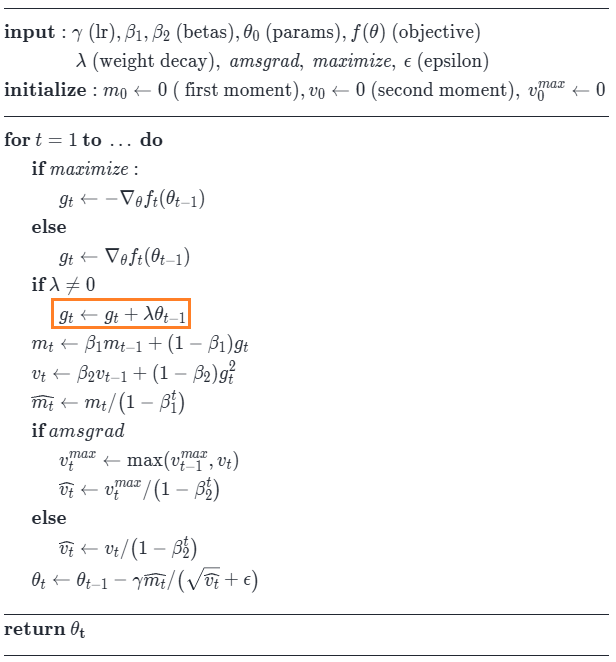
\includegraphics[width=0.75\textwidth]{Adam_formula}
\end{figure}

\newpage
\textit{\textbf{The difference between AdamW and Adam lies in the place of application of L2 regularization}} (weight decay). When standard Adam applies regularization directly to gradients (see step 1 of the calculation, which can lead to undesirable effects), \textit{\textbf{AdamW does this separately, at the parameter update level}}, and not at the gradient level. In this way, AdamW implements the weight decay concept more accurately, which can lead to better learning outcomes. In other words, an additional step is added to AdamW (replacing the moment with L2-regularization).
\\\\
\textit{\textbf{The AdamW algorithm:}}

0) Initially, at $t=0$, moments $m_t$ (or $m_0$) and $v_t$ (or $v_0$) for the weight matrices are zero.

1) The gradient $g_t$ (the derivative of the loss function with respect to the current weight $\theta$) is calculated using the formula:
    $$g_t = \nabla_{\theta}L(\theta_t)$$
    
2) The moments are updated (using exponential attenuation $\sim$ so that the "old" gradients are forgotten and the "new" ones have more weight):
    $$m_t = \beta_1 \cdot m_{t-1} + (1 - \beta_1) \cdot g_t$$
    $$v_t = \beta_2 \cdot v_{t-1} + (1 - \beta_2) \cdot g_t^2$$

    $\beta_1$ (usually 0.9) determines how much we trust past experience. $\beta_2$ (usually 0.999) is responsible for the "memory" of gradient volatility.
    
3) Bias Correction. Due to the fact that at the very beginning of training $m_t$ and $v_t$ are equal to 0, they "accelerate" for a long time and tend to zero. To fix this, they are scaled (due to which, for small $t>0$, their values are several times larger than they should be, but as $t$ increases, $\beta^t$ decreases, and therefore the scaling factor tends to 1):
    $$\hat{m}_t = \frac{m_t}{1-\beta_1^t}$$
    $$\hat{v}_t = \frac{v_t}{1-\beta_2^t}$$
    
4) \textbf{Regularization is applied to weights} $\theta$ ($\lambda$ is the regularization coefficient, weight decay):
    $$\theta_{t+1} = \theta_{t} - \eta \cdot \lambda \cdot \theta_{t}$$
    
5) The stage of updating the model weights ($\eta$ — learning rate, $\epsilon$ — minimum addition so that there is no zero in the denominator):
    $$\theta_{t+1} = \theta_{t+1} - \eta \cdot \frac{\hat{m}_t}{\sqrt{\hat{v}_t} + \epsilon}$$

    Steps 4 and 5 can be rewritten as follows:
    $$\theta_{t+1} = \theta_{t} - \eta \cdot \lambda \cdot \theta_{t} - \eta \cdot \frac{\hat{m}_t}{\sqrt{\hat{v}_t} + \epsilon} = \theta_{t} - \eta \cdot \left(\frac{\hat{m}_t}{\sqrt{\hat{v}_t} + \epsilon} + \lambda \cdot \theta_{t} \right)$$
\begin{figure}[h]
\centering
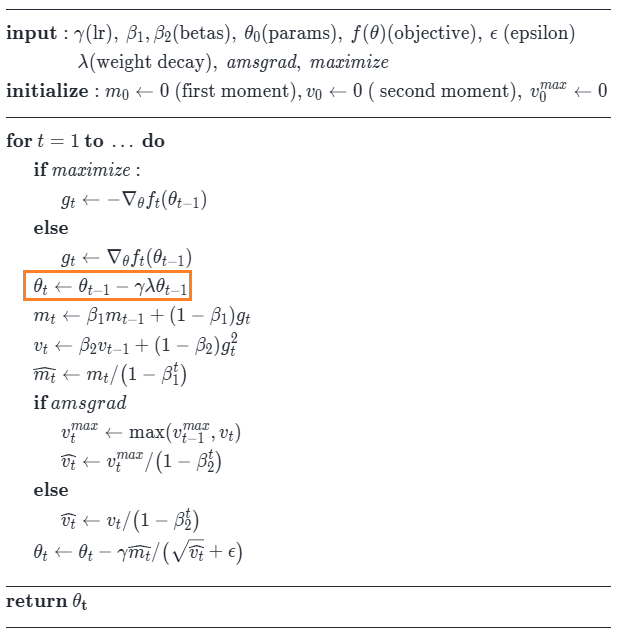
\includegraphics[width=0.75\textwidth]{AdamW_formula}
\end{figure}

Advantages of the AdamW optimizer:
\begin{itemize}
    \item Each parameter gets its own effective Learning Rate.
    \item Due to inertia ($m_t$), the algorithm wags less on noisy data.
    \item Adam usually converges faster than regular SGD and is less sensitive to the initial learning rate setting.
    \item Adam almost always works out of the box with default hyperparameters.
\end{itemize}


\newpage
\section{Muon}
The \textbf{Muon} Optimizer (Momentum Updated Orthogonalized Optimizer) is an algorithm for optimizing the weights of neural networks based on orthogonalization of gradients (bringing the gradient matrix to an orthogonal form, where each column and row are orthogonal (perpendicular) to each other and have a length of 1). While standard optimizers like Adam adapt the step for each weight separately (using the moving average of the square of the gradient), Muon works with entire parameter matrices, trying to make them "as informative as possible", without duplicating information and preserving the spectral properties of the weight matrices.

\textbf{Operating principle}: 
Ordinary gradients often contain redundancy, due to which many directions in the weight space are updated almost identically. Muon applies an operation to the gradient matrix that makes it orthogonal (or approximately orthogonal). Muon, like Adam, also uses Momentum ($m_t$, the moving average of the gradient), which helps to avoid getting stuck in local minima. But, unlike Adam, Muon does not store the moving average of the squares of the gradient to adapt the step, which reduces its memory requirements.
\\\\
\textit{\textbf{The Muon algorithm:}}

0) Initially, at $t=0$, the Momentum $m_t$ (or $m_0$) of the weight matrices is zero.

1) The gradient $g_t$ (the derivative of the loss function with respect to the current weight $\theta$) is calculated using the formula:
    $$g_t = \nabla_{\theta}L(\theta_t)$$
    
2) Consideration of Momentum, which makes it possible to smooth out noise and keep the inertia of movement (in a different way than in Adam) to a minimum of the loss function (coefficient $\mu$, in Adam it is $\beta_1$ $\sim$ how much do we trust past experience):
    $$m_t = \mu \cdot m_{t-1} + g_t$$

    If we use Nesterov's Momentum, then:
    $$m_t = \mu^2 \cdot m_{t-1} + (1 + \mu) \cdot g_t$$
    
3) Calculation of orthogonalization of the gradient matrix $O_t$, for which Muon takes the matrix of accumulated gradients and applies the Newton-Schultz iterative procedure to it to obtain an approximation (instead of the classical SVD decomposition, which is computationally expensive):
    $$O_t = NS_k^{(a,b,c)}(m_t; \epsilon)$$
    
    Here $(a,b,c)$ are the coefficients of the Newton-Schultz orthogonalization polynomial, $\epsilon$ is the minimum addition so that there is no zero in the denominator.
    
    Due to this, the product of the matrix itself is $OO^T \approx 1$, all singular values of the matrix become equal to 1, which removes the problem of different gradient scales for different layers and parameters.
    
4) \textbf{Appling L2 regularization to weights} ($\lambda$ is the regularization coefficient or weight decay, $\eta$ — initial learning rate):
    $$\theta_{t+1} = \theta_{t} - \eta \cdot \lambda \cdot \theta_{t}$$

5) Recalculation the update step $\eta$ (learning rate) depending on the dimension of the weight matrix (so that the orthogonalized update has a consistent RMS value for rectangular matrices) and taking into account the orthogonal gradient matrix for updating the weights:
    $$\eta = AdjustLR(\eta; shape(\theta_t))$$
    $$\theta_{t+1} = \theta_{t+1} - \eta \cdot O_t$$

    Steps 4 and 5 can be rewritten as follows:
    $$\theta_{t+1} = \theta_{t} - \eta \cdot \lambda \cdot \theta_{t} - AdjustLR(\eta; shape(\theta_t)) \cdot O_t$$

\begin{figure}[h]
\centering
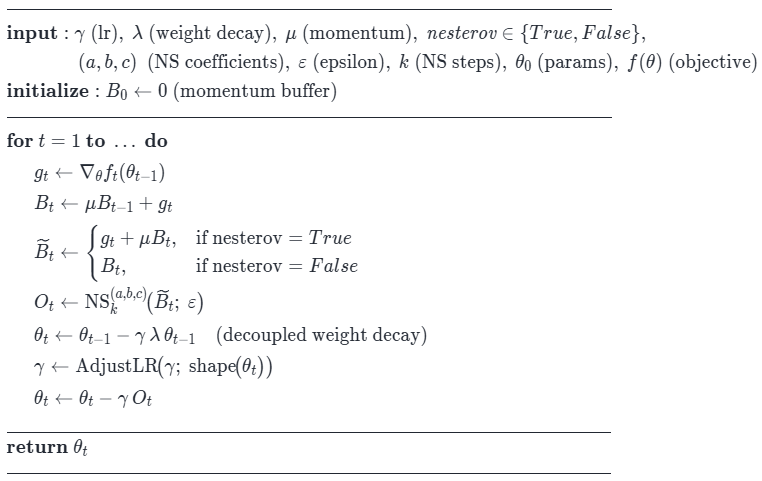
\includegraphics[width=0.75\textwidth]{Muon_formula}
\end{figure}

Advantages of the Muon optimizer:
\begin{itemize}
    \item Aligns the update scale in all singular directions (Muon forces all directions in the scale space to be trained at the same speed, whereas in Adam some directions can "fade out" faster than others).
    \item Accelerates convergence, as the optimizer does not waste time "rocking" in the narrow canyons of the loss function.
    \item Allows you to use a higher learning rate without losing stability.
    \item Requires less memory, as it stores only one moving average (for Momentum) instead of two.
\end{itemize}

Muon is designed specifically for \textbf{two-dimensional weight matrices} (linear layers), while AdamW is usually used for the rest of the parameters (embedding, normalization, bias).



\chapter{Fine-tuning results}
For the correctness of the comparison, the following hyperparameters were set for all fine-tuning experiments:
\begin{itemize}
    \item Maximum number of samples: 4000
    \item Test proportion: 10\%
    \item Additional validation during training on benchmarks: "piqa", "winogrande"
    \item Limit on the number of tokens generated by the model: 256
    \item Maximum number of training epochs: 20
    \item Epochs before early stopping of training (without improving the tracked metric and/or convergence of weights): 3
    \item Tracked metric for training early stopping: AVG Accuracy on benchmarks
    \item Initial learning rate: $2 \cdot 10^{-5}$
    \item Learning scheduler that changes the learning rate 0.5 times every 4 epochs
    \item L2 regularization coefficient to prevent overfitting: 0.1
    \item Momentum coefficient: 0.9
    \item Batch size: 4
    \item Random seed: 42
\end{itemize}

Changing some of hyperparameters can affect the training and convergence process both for the better (increasing the batch size for Muon acceleration, since it consumes less memory) and for the worse (reducing the learning rate, to which Muon is highly sensitive, will lead to a significant decrease in the steps of changing weights and, consequently, slowing down the updating of weights).

\newpage
\section{AdamW results}
\noindent
\begin{figure}[h]
\centering
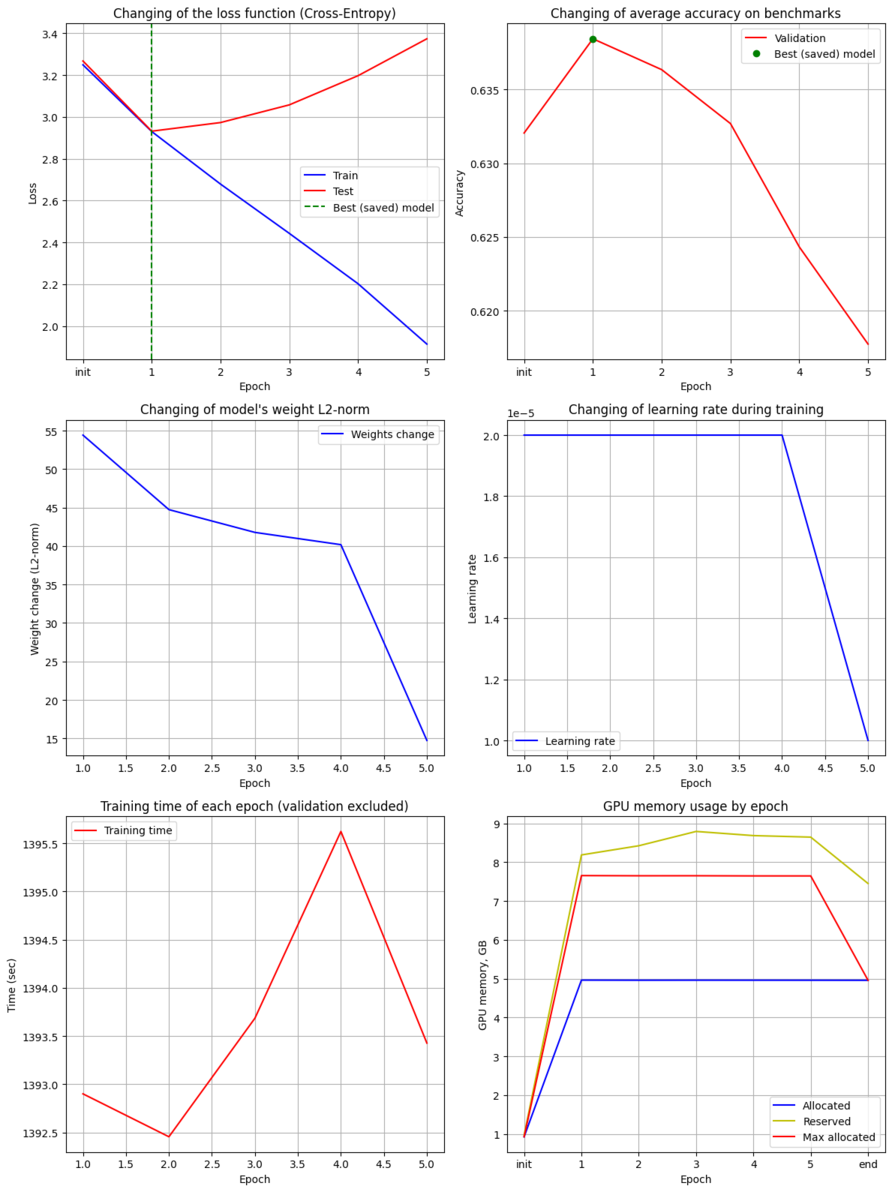
\includegraphics[width=0.7\textwidth]{AdamW_finetuning_results}
\end{figure}

\newpage
\section{Muon results}
\noindent
\begin{figure}[h]
\centering
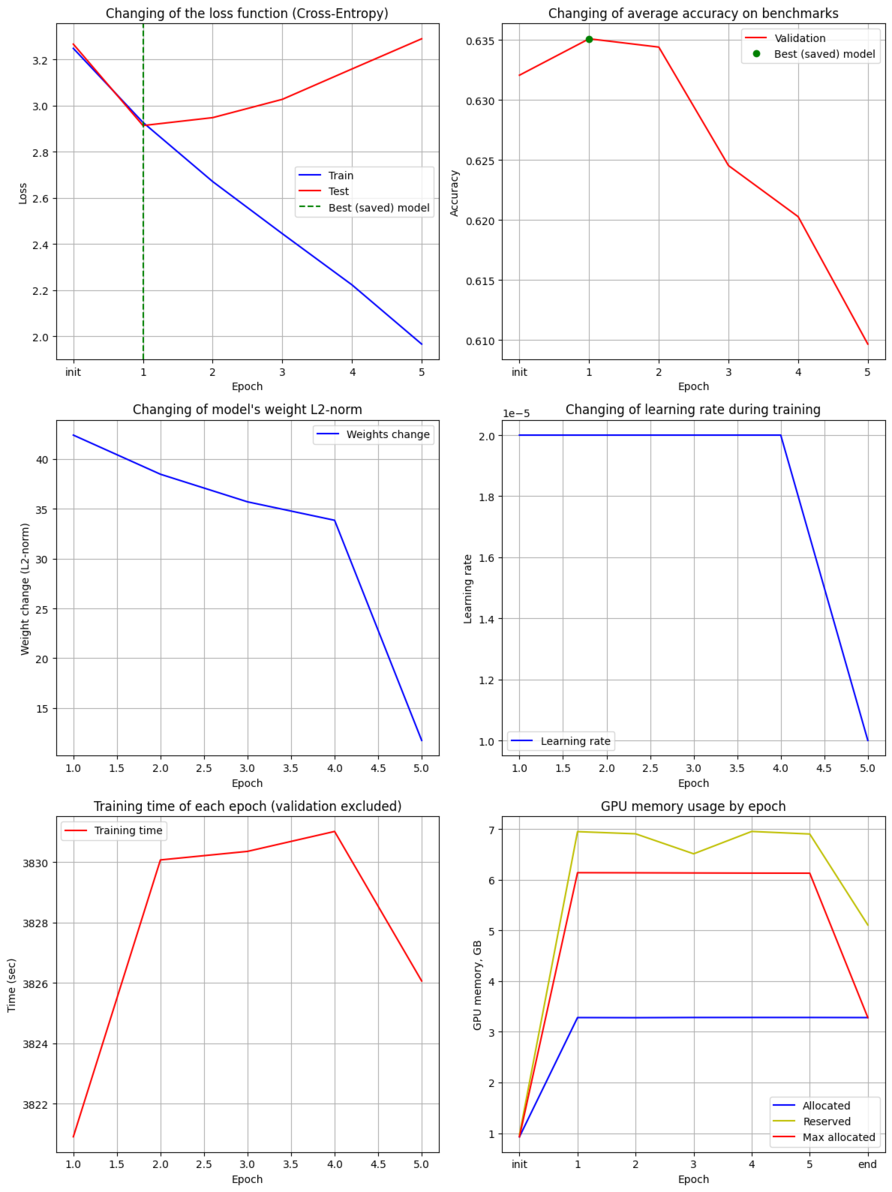
\includegraphics[width=0.7\textwidth]{Muon_finetuning_results}
\end{figure}

\newpage
\section{Muon with AdamW results}
\noindent
\begin{figure}[h]
\centering
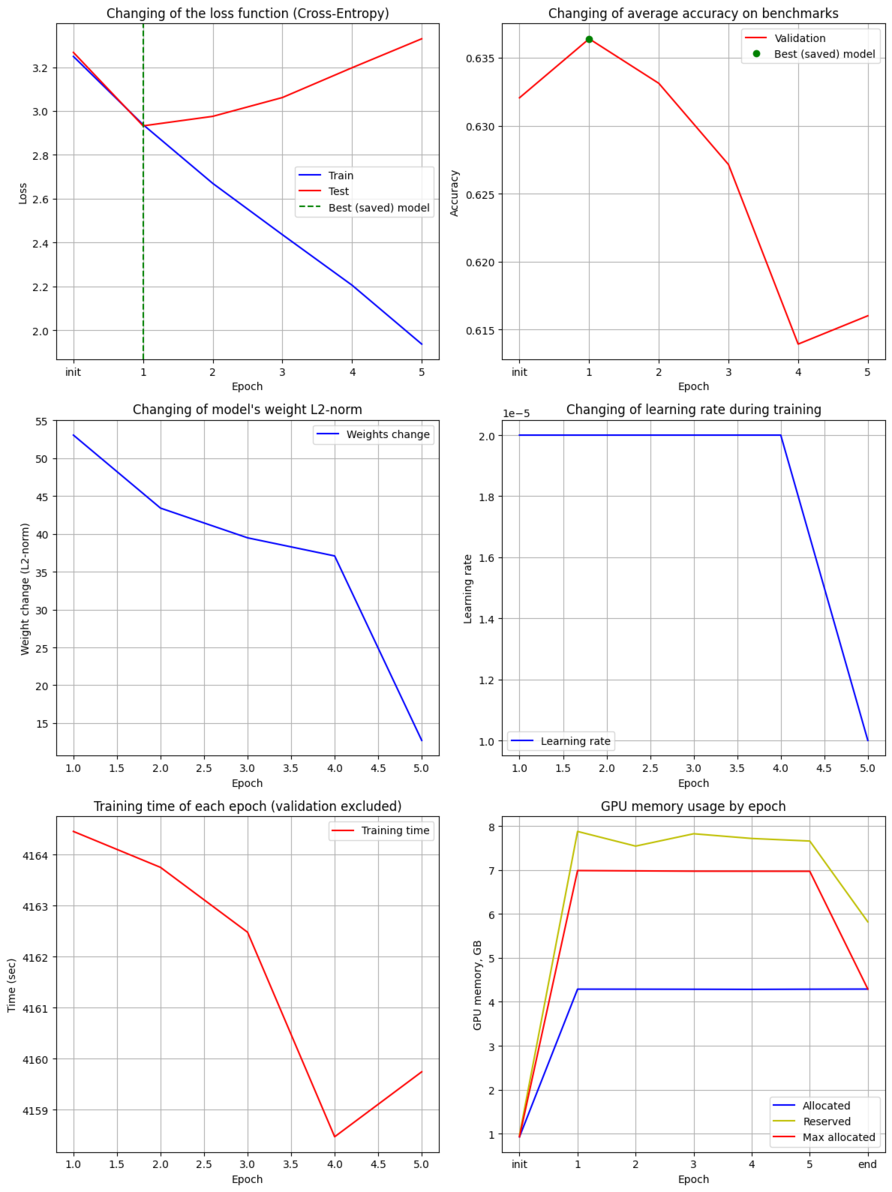
\includegraphics[width=0.7\textwidth]{Muon_with_AdamW_finetuning_results}
\end{figure}



\chapter{Results comparison}
For a more comprehensive analysis, another experiment was conducted, which included 8000 samples instead of 4000. The training was only with AdamW optimizer (\textit{AdamW\_8k}), since other optimizers simply did not fit into the Kaggle quota.


\section{Cross-Entropy Loss}
\noindent
\begin{figure}[h]
\centering
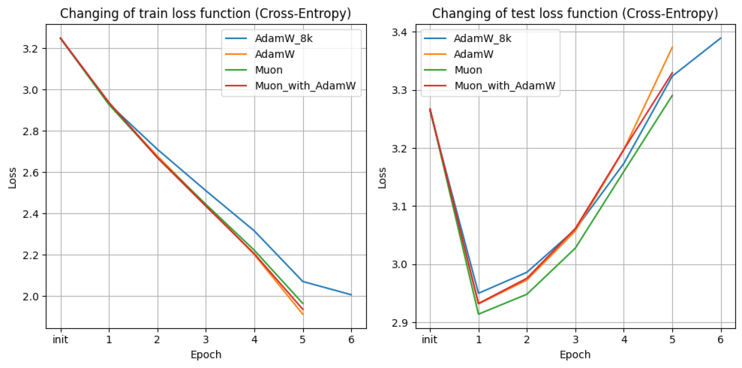
\includegraphics[width=1\textwidth]{comparison_loss}
\end{figure}

When fine-tuning with any optimizer (\textit{including AdamW\_8k experiment}), the \textbf{change in Cross-Entropy loss}, both on training data and on test data, has approximately the \textit{\textbf{same trend. Fast learning with a strong loss decrease on train data, but at the same time overfitting after the first epoch}} (loss on test data has a V-shaped trend). This observation can be explained by the fact that the model is too large for such a small amount of disparate data (even increasing to 8000 samples did not solve the problem).


\section{Average accuracy on benchmarks subset}
\noindent
\begin{figure}[h]
\centering
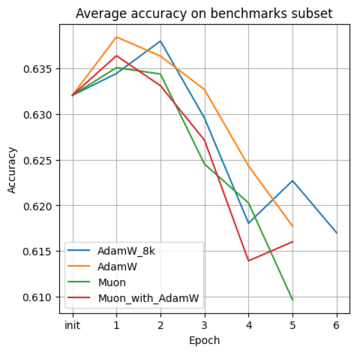
\includegraphics[width=0.7\textwidth]{comparison_accuracy}
\end{figure}

The \textbf{change in tracked metric} (\textit{average accuracy on subset of benchmarks}) also shows a similar \textit{\textbf{trend among all experiments, where the metric improves at 1-2 epochs, after which there is a sharp decline due to overfitting}}. At the same time, training with AdamW (\textit{AdamW, AdamW\_8k, Muon\_with\_AdamW experiments}) shows slightly higher accuracy than when training only with the Muon optimizer (\textit{it should be clarified that only 72\% of the model weights are trained in Muon, whereas in other experiments all 100\%}).


\newpage
\section{Training time and convergence}
\begin{figure}[h]
\centering
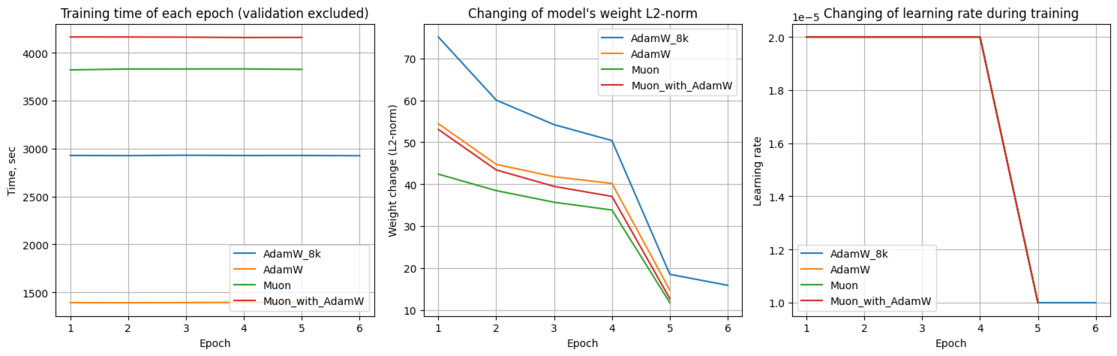
\includegraphics[width=1\textwidth]{comparison_training_time_and_weight_convergence}
\end{figure}

\noindent \textbf{Training time} varies greatly between optimizers, where:
\begin{enumerate}
    \item \textit{\textbf{AdamW optimizer are the fastest}} (even with twice the amount of input data), $\sim$1400 seconds per 4000 samples (23 minutes per epoch) and $\sim$3000 seconds (50 minutes per epoch with 8000 samples). The training time depends almost linearly on the amount of data.
    \item \textit{\textbf{Muon}} optimizer, even with only 4000 samples, spent $\sim$3,800 seconds per epoch, which is just over an hour and which is almost \textit{\textbf{3 times worse than AdamW}} on the same data.
    \item \textit{\textbf{Combination of Muon with AdamW showed the longest training time}} ($\sim$4100 seconds), since optimization of other weight matrices using AdamW was added on top to the weight optimization with Muon.
\end{enumerate}

\noindent \textbf{L2 norm of change in weights} during training also varies. 
\begin{enumerate}
    \item \textit{\textbf{Weights changed the least when optimized by the Muon algorithm}}, while the value of loss function was comparable to other optimizers. That is, to achieve similar "progress", it is enough for Muon optimizer  to change a smaller number of weights (only 72\% are trained, not 100\%) and to a lower value (\textit{while the loss on the test data is even better than that of other optimizers, which cannot be said about the accuracy on benchmarks}). 
    \item \textit{\textbf{The weights changed the most when training with AdamW}}, with a 25\% more pronounced shift in relation to Muon.
    \item Changing the weights with a \textit{\textbf{combination of optimizers turned out to be something in between Muon and AdamW}}.
\end{enumerate}

\textit{It is also worth to note that with more data, the more the weights of the model changed (according to experiments with 4000 and 8000 samples).}
\clearpage
\begin{figure}[h]
\centering
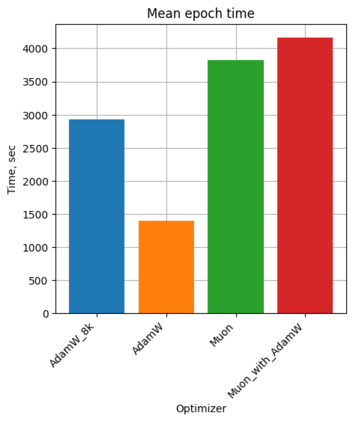
\includegraphics[width=0.6\textwidth]{comparison_mean_time}
\end{figure}
\begin{figure}[h]
\centering
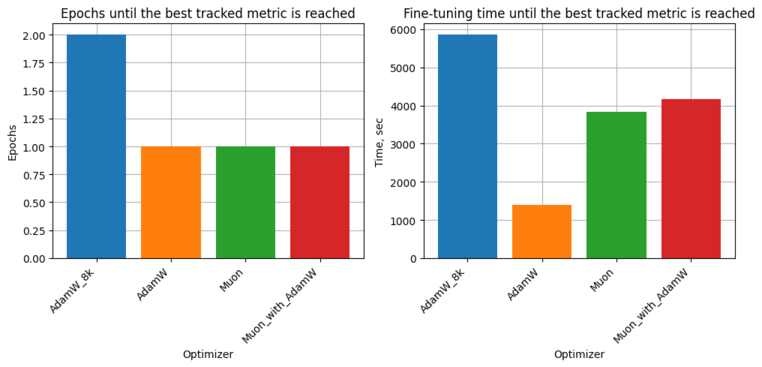
\includegraphics[width=0.9\textwidth]{comparison_epochs_best}
\end{figure}
\textit{\textbf{It took only one epoch for the models to be fine-tuned to the best accuracy on the benchmarks}} at 4000 samples. \textit{If training on more data, then along with the increase of computing time, the accuracy will also be higher.}


\clearpage
\section{GPU memory usage}
\begin{figure}[h]
\centering
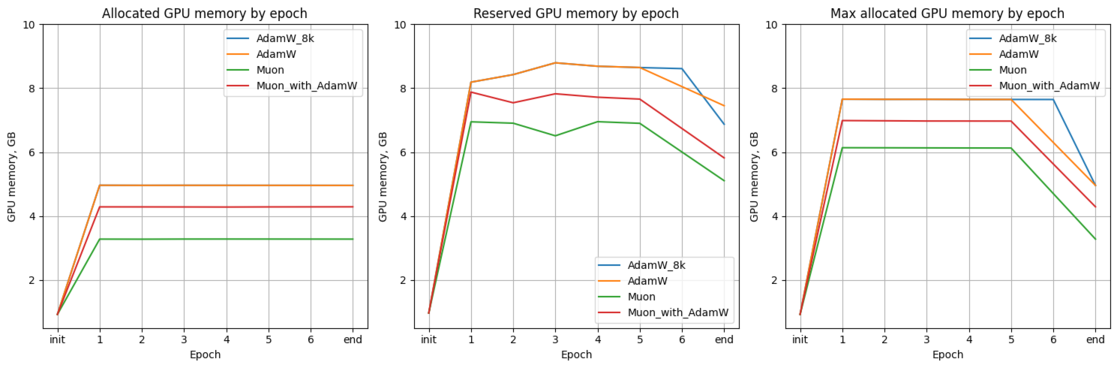
\includegraphics[width=1\textwidth]{comparison_gpu_memory}
\end{figure}

Between epochs, GPU memory usage remains almost unchanged (for each optimizer), so proceed to consider the average value of GPU usage.

\begin{figure}[h]
\centering
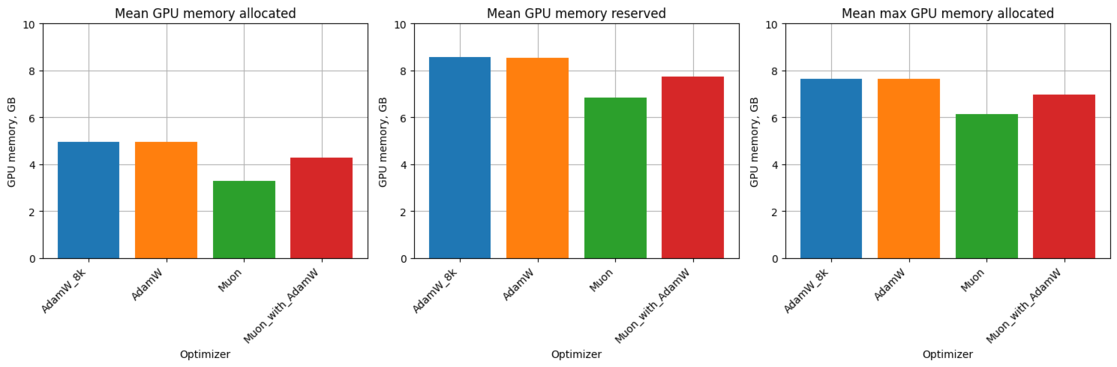
\includegraphics[width=1\textwidth]{comparison_gpu_memory_mean}
\end{figure}

Memory usage depends only on the type of optimizer and does not depend on the dataset size (since only a fixed-size batch is loaded at one time).
\\\\
\noindent GPU allocated memory after an epoch:
\begin{itemize}
    \item \textit{\textbf{The highest for the AdamW optimizer}}, since it stores two moments at once for each trainable weights (the moving average of the gradients and the moving average of the squares of the gradients). It takes up 4.96 GB with the model.
    \item After one fine-tuning epoch, \textit{\textbf{Muon frees up more memory}}, by about 33\%, compared to AdamW. Occupying only 3.28 GB with the model.
    \item \textit{\textbf{Combination of Muon and AdamW has average consumption}} (4.29 GB), after training they take up 15\% less memory compared to AdamW, and 30\% more when compared with only Muon.
\end{itemize}

\noindent Reserved (cached) GPU memory:
\begin{itemize}
    \item Similarly, AdamW optimizer reserves the most memory, 8.55 GB.
    \item One Muon reserves 20\% less memory (6.84 GB).
    \item The combination of optimizers again has an intermediate value (7.73 GB), 10\% less than AdamW, but 13\% more than Muon.
\end{itemize}

\noindent \textbf{Maximum GPU allocated memory during training epoch}:
\begin{itemize}
    \item \textit{\textbf{AdamW has the highest}}, 7.65 GB.
    \item \textit{\textbf{Muon consumes 20\% less GPU memory}} (6.13 GB) than AdamW during training.
    \item The optimizer combination consumes 6.98 GB, which is 9\% less and 14\% more than AdamW and Muon, respectively.
\end{itemize}


\section{Benchmarks}
Validation data is the following datasets that evaluate the understanding of the model of physical properties and logical relationships between objects, as well as the possibilities of commonsense reasoning:
\begin{enumerate}
    \item \href{https://github.com/EleutherAI/lm-evaluation-harness/tree/main/lm_eval/tasks/piqa}{PIQA} (Physical Interaction: Question Answering) — benchmark for determining how well a language model understands the physical properties of objects (\textit{fragility, hardness*) and everyday actions (*how best to wash dishes or place an object}). 
    \item \href{https://github.com/EleutherAI/lm-evaluation-harness/tree/main/lm_eval/tasks/arc}{ARC easy} (AI2 Reasoning Easy) — benchmark created to evaluate the ability of artificial intelligence systems to answer questions that require basic scientific knowledge and logic. The set consists of multiple-answer questions taken from real school science exams (grades 3-9). The "Easy" category includes questions that modern (at the time of creation) models could answer using simple statistical methods or keyword search.
    \item \href{https://github.com/EleutherAI/lm-evaluation-harness/tree/main/lm_eval/tasks/arc}{ARC challenge} (AI2 Reasoning Challenge) — structurally similar to "ARC easy", but contains more difficult questions that require "multi-layered" reasoning to answer.
    \item \href{https://github.com/EleutherAI/lm-evaluation-harness/tree/main/lm_eval/tasks/winogrande}{WinoGrande} — benchmark designed to evaluate the ability of artificial intelligence models to reason based on common sense (commonsense reasoning). The benchmark is based on tasks like the Winograd Schema Challenge (WSC), where the model needs to correctly correlate a pronoun with one of two objects mentioned in the sentence. For example, there is an expression "The trophy did not fit in a brown suitcase because *** was too big." The model needs to choose correct answer from a suggested ones. Options: A) Trophy; B) Suitcase. The correct answer is: A (Trophy).
    \item \href{https://github.com/EleutherAI/lm-evaluation-harness/tree/main/lm_eval/tasks/hellaswag}{HellaSwag} (Harder Entities, Longer Contexts, and Better Adversarial Filtering) — benchmark created to evaluate the commonsense reasoning abilities of large language models (LLM). The benchmark checks how well the model can predict the most logical outcome of an everyday scenario. Unlike simple tests, HellaSwag uses the Adversarial Filtering method: the answer options are generated so that they look plausible to algorithms, but are obviously incorrect to humans. The model gets a context (for example, a description of the beginning of a video clip) and four continuation options. The task is to choose the right one. Tasks are chosen so that they are easy for humans (accuracy $\sim$ 95\%), but for a long time remained extremely difficult for AI.
\end{enumerate}

The main metric of all benchmarks is \textbf{Accuracy}, that is, the indexes of answers predicted by a model (0, 1, ...) are compared with true label. The higher the Accuracy, the better the model understands essence of the sentence. To do this, CausalLM model is used to estimate logarithmic probability (log-likelihood) of each of the response options. The model "chooses" option that is more likely to be generated with a given context (input).

\begin{figure}[h]
\centering
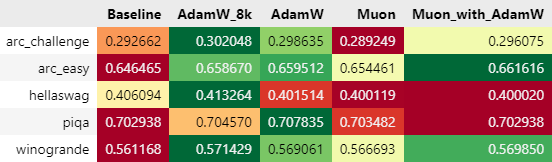
\includegraphics[width=1\textwidth]{comparison_benchmarks}
\end{figure}
\noindent Comparing \textbf{Accuracy on benchmarks}, it can be seen that:
\begin{itemize}
    \item  \textit{\textbf{The best metrics, as expected, were shown by experiment with the largest number of samples}} (8000 versus 4000 for all other optimizers). It surpassed the "baseline" (model without fine-tuning) in all benchmarks by 0.2 — 1.2\% Accuracy. 
    \item  \textit{\textbf{AdamW}}, trained on 4,000 samples, \textit{\textbf{ranks second}} in terms of Accuracy. He even managed to slightly (by $\sim$0.001 — 0.003, which is less than half a percent) overtake AdamW\_8k on "arc\_easy" and "piqa" benchmarks.
    \item  \textit{\textbf{The combination of optimizers showed the most unstable metrics}}, for benchmarks "arc\_easy" and "winogrande" there is a relatively good increase in Accuracy, while for "hellaswag" and "piqa" model performed worse than its untrained version.
    \item  \textit{\textbf{One Muon showed the worst results}}, in two benchmarks it was worse than untrained model ("arc\_challenge" and "hellaswag"), and in the other three it was only slightly better ("arc\_easy", "piqa", "winogrande").
\end{itemize}



\chapter{Conclusion}
\textbf{Key Findings}:
\begin{itemize}
    \item The \textit{\textbf{final quality of a model is more influenced by amount of data than a type of optimizer }}(\textit{although fune-tuning with Muon showed almost no improvement in Accuracy}).
    \item The \textit{\textbf{convergence of models with respect to the loss function is almost the same for optimizers}}, but not according to L2 norm of updated model's weights, they change the most with AdamW optimizer, the weakest with Muon since not all parameters are trained (\textit{while their loss is almost the same}).
    \item \textit{\textbf{Muon is running much slower}} (\textit{3 times}) than AdamW (\textit{although this may be due to the architecture of a model}).
    \item \textit{\textbf{Muon requires less memory}} (\textit{by $\sim$20\% compared to AdamW}), as it stores only one additional matrix for weights (Momentum) and it doesn't fine-tune all the parameters.
    \item There are perspectives for Muon related to increasing the batch size and learning rate.
    \item \textit{\textbf{The combination of optimizers shows intermediate results}} in all analysis, except for training time, where fine-tuning took the longest.
\end{itemize}

\noindent \textbf{Opportunities for further research}:
\begin{itemize}
    \item Using the MeZO optimizer;
    \item Training on full dataset;
    \item Using a model for which orthogonalization of matrices would be more profitable and faster than calculating gradients;
    \item Increase the learning rate and batch size.
\end{itemize}


\end{document}
